\documentclass[../thesis.tex]{subfiles}

\begin{document}

\chapter{Methodology}
\label{chap:method}

\noindent In this chapter we present the methodology and research structure used in this thesis. Some pre-processing of data including imputation and dimensional reduction will also be explained and presented. The implementation of the ML algorithms that produce the results presented in chapter (\ref{chap:exp}) are also mentioned, with the source code being found in appendix (\ref{chap:souce_code}). 

\section{Overview}

\noindent As stated in the chapter (\ref{chap:intro}), the aim of the thesis is split into two parts. The first part being that of seeing how well various clustering methods perform in producing phenotypically distinct clinical patient groups with HFpEF and HFmrEF? We frame the SL problem in the setting of unsupervised learning and accordingly use the following clustering methods: hierarchical clustering, expectation-maximization and latent class analysis to evaluate which produce the most clinically useful patient groups. The use of these clustering methods are common in the literature (see section \ref{subsec:unsupervisedlearn}) and serves as the main motivation for including them in our analysis. The second part of the problem statement looks at evaluating the accuracy of various classification algorithms in predicting the mortality and re-admission of patients with HFpEF and HFmrEF? In accordance with the literature as presented in section (\ref{sec:predclincout}), we reduce the SL problem of predicting the mortality and re-admission into a two class classification problem where both classes of outcomes are whether or not mortality/re-admission  
\begin{figure}

\centering
\small






\tikzset{every picture/.style={line width=0.75pt}} %set default line width to 0.75pt        

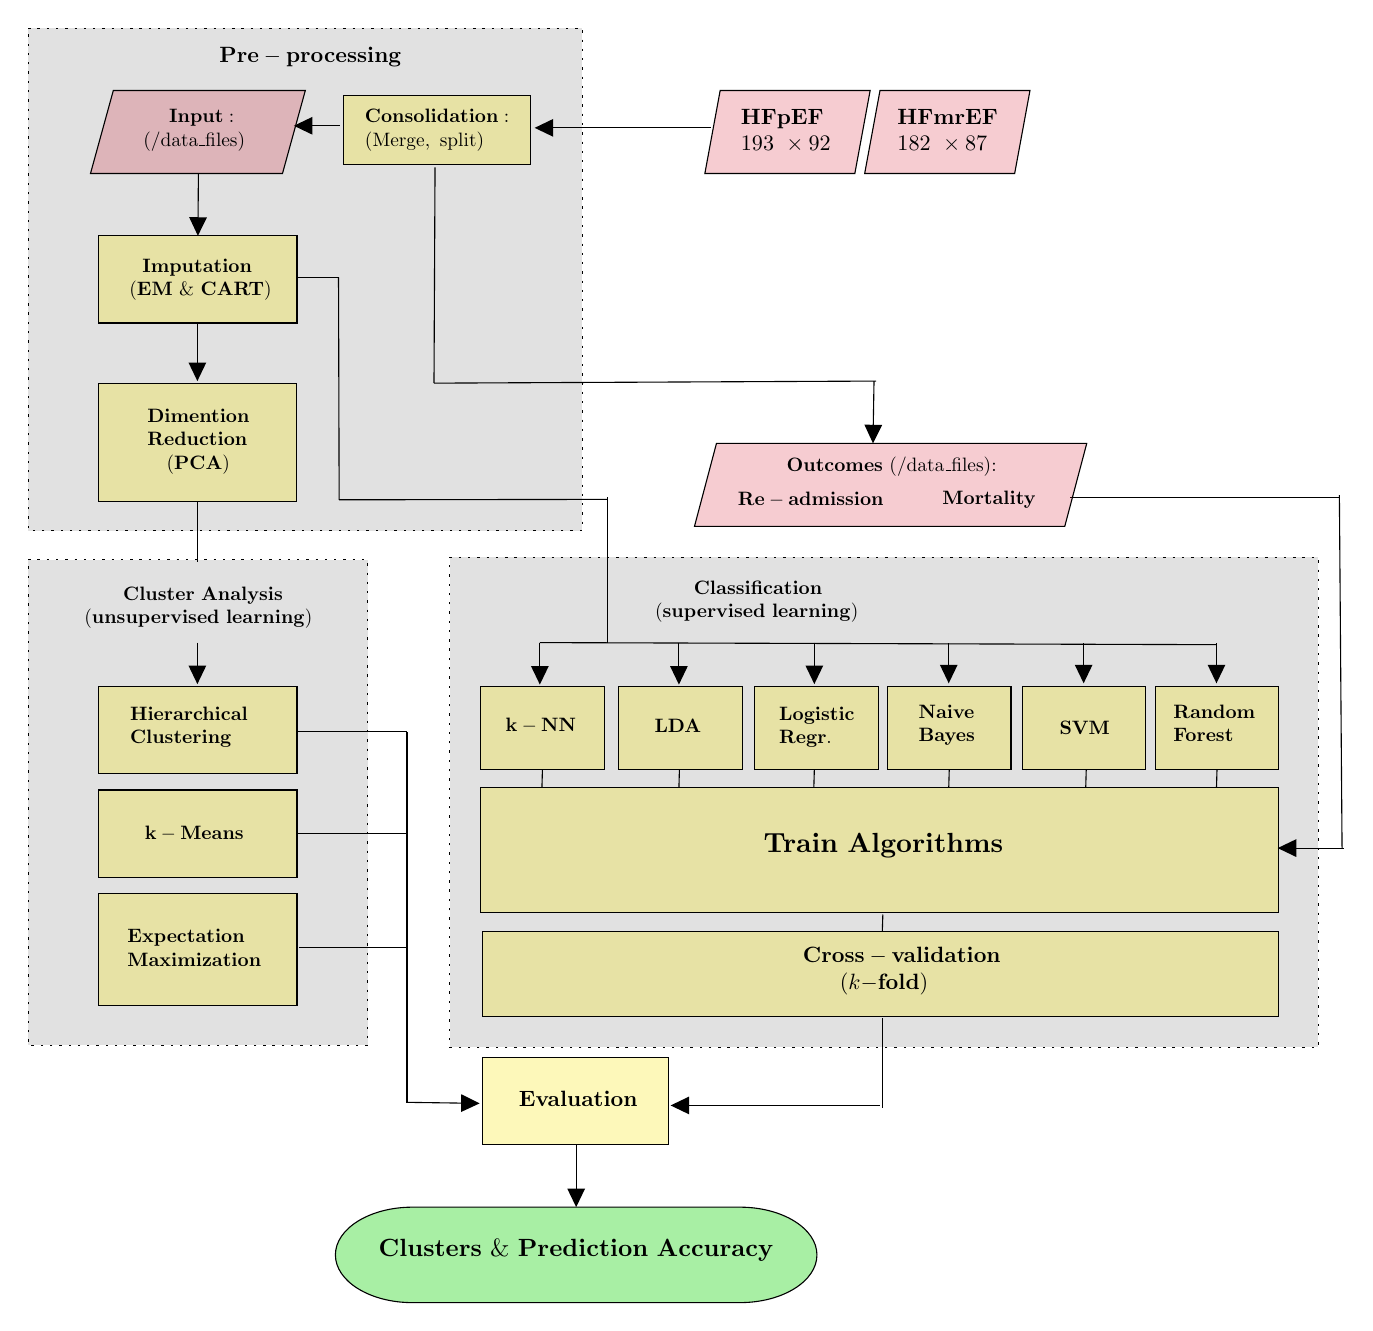
\begin{tikzpicture}[x=0.75pt,y=0.75pt,yscale=-1,xscale=1]
%uncomment if require: \path (0,646); %set diagram left start at 0, and has height of 646

%Shape: Rectangle [id:dp17767432122865645] 
\draw  [fill={rgb, 255:red, 155; green, 155; blue, 155 }  ,fill opacity=0.3 ][dash pattern={on 0.84pt off 2.51pt}] (2,5) -- (269,5) -- (269,247) -- (2,247) -- cycle ;
%Shape: Rectangle [id:dp17276791081063103] 
\draw  [fill={rgb, 255:red, 155; green, 155; blue, 155 }  ,fill opacity=0.3 ][dash pattern={on 0.84pt off 2.51pt}] (205,260) -- (623.5,260) -- (623.5,496) -- (205,496) -- cycle ;
%Shape: Rectangle [id:dp137712763597037] 
\draw  [fill={rgb, 255:red, 155; green, 155; blue, 155 }  ,fill opacity=0.3 ][dash pattern={on 0.84pt off 2.51pt}] (2,261) -- (165.5,261) -- (165.5,495) -- (2,495) -- cycle ;
%Straight Lines [id:da9350378875346577] 
\draw    (84,75) -- (83.77,103) ;
\draw [shift={(83.75,105)}, rotate = 270.48] [fill={rgb, 255:red, 0; green, 0; blue, 0 }  ][line width=0.75]  [draw opacity=0] (8.93,-4.29) -- (0,0) -- (8.93,4.29) -- cycle    ;

%Straight Lines [id:da9986924600189169] 
\draw    (83.5,147) -- (83.5,173) ;
\draw [shift={(83.5,175)}, rotate = 270] [fill={rgb, 255:red, 0; green, 0; blue, 0 }  ][line width=0.75]  [draw opacity=0] (8.93,-4.29) -- (0,0) -- (8.93,4.29) -- cycle    ;

%Straight Lines [id:da9104422198905568] 
\draw    (184.5,344) -- (184.5,523) ;


%Straight Lines [id:da17863107757037655] 
\draw    (184.5,522.5) -- (217.5,522.97) ;
\draw [shift={(219.5,523)}, rotate = 180.82] [fill={rgb, 255:red, 0; green, 0; blue, 0 }  ][line width=0.75]  [draw opacity=0] (8.93,-4.29) -- (0,0) -- (8.93,4.29) -- cycle    ;

%Straight Lines [id:da4423537570819638] 
\draw    (248.5,301) -- (248.5,319.22) ;
\draw [shift={(248.5,321.22)}, rotate = 270] [fill={rgb, 255:red, 0; green, 0; blue, 0 }  ][line width=0.75]  [draw opacity=0] (8.93,-4.29) -- (0,0) -- (8.93,4.29) -- cycle    ;

%Straight Lines [id:da14828368689404448] 
\draw    (315.5,301) -- (315.5,319.22) ;
\draw [shift={(315.5,321.22)}, rotate = 270] [fill={rgb, 255:red, 0; green, 0; blue, 0 }  ][line width=0.75]  [draw opacity=0] (8.93,-4.29) -- (0,0) -- (8.93,4.29) -- cycle    ;

%Straight Lines [id:da2745541849199835] 
\draw    (380.75,301) -- (380.75,319) ;
\draw [shift={(380.75,321)}, rotate = 270] [fill={rgb, 255:red, 0; green, 0; blue, 0 }  ][line width=0.75]  [draw opacity=0] (8.93,-4.29) -- (0,0) -- (8.93,4.29) -- cycle    ;

%Straight Lines [id:da10622223865111557] 
\draw    (445.5,301.39) -- (445.5,318.61) ;
\draw [shift={(445.5,320.61)}, rotate = 270] [fill={rgb, 255:red, 0; green, 0; blue, 0 }  ][line width=0.75]  [draw opacity=0] (8.93,-4.29) -- (0,0) -- (8.93,4.29) -- cycle    ;

%Straight Lines [id:da12728372488873485] 
\draw    (248.5,301) -- (574.5,302) ;


%Straight Lines [id:da04201945911359806] 
\draw    (413.5,482) -- (413.5,525) ;


%Straight Lines [id:da8309940078541183] 
\draw    (313.5,524) -- (412.5,524) ;

\draw [shift={(311.5,524)}, rotate = 0] [fill={rgb, 255:red, 0; green, 0; blue, 0 }  ][line width=0.75]  [draw opacity=0] (8.93,-4.29) -- (0,0) -- (8.93,4.29) -- cycle    ;
%Shape: Rectangle [id:dp805733141303524] 
\draw  [fill={rgb, 255:red, 248; green, 231; blue, 28 }  ,fill opacity=0.3 ] (220,371) -- (604.5,371) -- (604.5,431) -- (220,431) -- cycle ;
%Straight Lines [id:da5772744105119383] 
\draw    (281,231) -- (281,301) ;


%Straight Lines [id:da5307166780329797] 
\draw    (504,231) -- (634,231) ;


%Straight Lines [id:da8350224251535634] 
\draw    (633.71,230) -- (635,400) ;


%Shape: Rectangle [id:dp7689144799085996] 
\draw  [fill={rgb, 255:red, 248; green, 231; blue, 28 }  ,fill opacity=0.3 ] (36,105) -- (131.5,105) -- (131.5,147) -- (36,147) -- cycle ;
%Shape: Rectangle [id:dp8360402522569712] 
\draw  [fill={rgb, 255:red, 248; green, 231; blue, 28 }  ,fill opacity=0.3 ] (35.75,176) -- (131.25,176) -- (131.25,233) -- (35.75,233) -- cycle ;
%Shape: Rectangle [id:dp8436521642341313] 
\draw  [fill={rgb, 255:red, 248; green, 231; blue, 28 }  ,fill opacity=0.3 ] (36,322) -- (131.5,322) -- (131.5,364) -- (36,364) -- cycle ;
%Shape: Rectangle [id:dp8779924325569846] 
\draw  [fill={rgb, 255:red, 248; green, 231; blue, 28 }  ,fill opacity=0.3 ] (36,372) -- (131.5,372) -- (131.5,414) -- (36,414) -- cycle ;
%Shape: Rectangle [id:dp8944427225779763] 
\draw  [fill={rgb, 255:red, 248; green, 231; blue, 28 }  ,fill opacity=0.3 ] (36,422) -- (131.5,422) -- (131.5,476) -- (36,476) -- cycle ;
%Straight Lines [id:da12044404667160191] 
\draw    (131.5,344) -- (184.5,344) ;


%Straight Lines [id:da6084938483975053] 
\draw    (131.5,393) -- (184.5,393) ;


%Straight Lines [id:da16731103541967607] 
\draw    (132.5,448) -- (184.5,448) ;


%Straight Lines [id:da9753125405011336] 
\draw    (151.8,232.2) -- (281,232) ;


%Straight Lines [id:da8528567916678871] 
\draw    (151.5,125) -- (151.8,232.2) ;


%Straight Lines [id:da9889731806347037] 
\draw    (131.5,125) -- (151.5,125) ;


%Shape: Rectangle [id:dp8708975358842101] 
\draw  [fill={rgb, 255:red, 248; green, 231; blue, 28 }  ,fill opacity=0.3 ] (220,322) -- (279.5,322) -- (279.5,362) -- (220,362) -- cycle ;
%Shape: Rectangle [id:dp2832466894461272] 
\draw  [fill={rgb, 255:red, 248; green, 231; blue, 28 }  ,fill opacity=0.3 ] (286.5,322) -- (346,322) -- (346,362) -- (286.5,362) -- cycle ;
%Shape: Rectangle [id:dp14049594498977225] 
\draw  [fill={rgb, 255:red, 248; green, 231; blue, 28 }  ,fill opacity=0.3 ] (352,322) -- (411.5,322) -- (411.5,362) -- (352,362) -- cycle ;
%Shape: Rectangle [id:dp4503091833898072] 
\draw  [fill={rgb, 255:red, 248; green, 231; blue, 28 }  ,fill opacity=0.3 ] (416,322) -- (475.5,322) -- (475.5,362) -- (416,362) -- cycle ;
%Straight Lines [id:da37279512049375874] 
\draw    (249.5,371) -- (249.75,362) ;


%Straight Lines [id:da7877038245504153] 
\draw    (315.5,371) -- (315.75,362) ;


%Straight Lines [id:da47196717706905766] 
\draw    (380.5,371) -- (380.75,362) ;


%Straight Lines [id:da6265135418883228] 
\draw    (445.5,371) -- (445.75,362) ;


%Shape: Rectangle [id:dp23123927252195697] 
\draw  [fill={rgb, 255:red, 248; green, 231; blue, 28 }  ,fill opacity=0.3 ] (221,440) -- (604.5,440) -- (604.5,481) -- (221,481) -- cycle ;
%Straight Lines [id:da6647772541294572] 
\draw    (83.5,233) -- (83.5,262) ;


%Straight Lines [id:da7585523119166355] 
\draw    (413.5,440) -- (413.75,432) ;


%Straight Lines [id:da49016539083231736] 
\draw    (266,543) -- (266,571) ;
\draw [shift={(266,573)}, rotate = 270] [fill={rgb, 255:red, 0; green, 0; blue, 0 }  ][line width=0.75]  [draw opacity=0] (8.93,-4.29) -- (0,0) -- (8.93,4.29) -- cycle    ;

%Shape: Parallelogram [id:dp518581715076881] 
\draw  [fill={rgb, 255:red, 208; green, 2; blue, 27 }  ,fill opacity=0.2 ] (335.38,35) -- (407.64,35) -- (400.26,75) -- (328,75) -- cycle ;
%Straight Lines [id:da992949141941001] 
\draw    (83.5,301) -- (83.5,319) ;
\draw [shift={(83.5,321)}, rotate = 270] [fill={rgb, 255:red, 0; green, 0; blue, 0 }  ][line width=0.75]  [draw opacity=0] (8.93,-4.29) -- (0,0) -- (8.93,4.29) -- cycle    ;

%Straight Lines [id:da6160084227975695] 
\draw    (197.5,176) -- (410.5,175) ;


%Straight Lines [id:da3499925619434392] 
\draw    (409.5,175) -- (409.03,203) ;
\draw [shift={(409,205)}, rotate = 270.95] [fill={rgb, 255:red, 0; green, 0; blue, 0 }  ][line width=0.75]  [draw opacity=0] (8.93,-4.29) -- (0,0) -- (8.93,4.29) -- cycle    ;

%Straight Lines [id:da2578176252932385] 
\draw    (197.5,176) -- (198,72) ;


%Straight Lines [id:da924957907848829] 
\draw    (132,52) -- (152,52) ;

\draw [shift={(130,52)}, rotate = 0] [fill={rgb, 255:red, 0; green, 0; blue, 0 }  ][line width=0.75]  [draw opacity=0] (8.93,-4.29) -- (0,0) -- (8.93,4.29) -- cycle    ;
%Straight Lines [id:da09848220518746698] 
\draw    (248,53) -- (331,53) ;

\draw [shift={(246,53)}, rotate = 0] [fill={rgb, 255:red, 0; green, 0; blue, 0 }  ][line width=0.75]  [draw opacity=0] (8.93,-4.29) -- (0,0) -- (8.93,4.29) -- cycle    ;
%Shape: Parallelogram [id:dp8152627621795523] 
\draw  [fill={rgb, 255:red, 208; green, 2; blue, 27 }  ,fill opacity=0.2 ] (43,35) -- (135.5,35) -- (124.5,75) -- (32,75) -- cycle ;
%Shape: Parallelogram [id:dp9253495901859852] 
\draw  [fill={rgb, 255:red, 208; green, 2; blue, 27 }  ,fill opacity=0.2 ] (333.6,205) -- (512,205) -- (501.4,245) -- (323,245) -- cycle ;
%Shape: Parallelogram [id:dp42719482691252253] 
\draw  [fill={rgb, 255:red, 208; green, 2; blue, 27 }  ,fill opacity=0.2 ] (412.38,35) -- (484.64,35) -- (477.26,75) -- (405,75) -- cycle ;
%Flowchart: Terminator [id:dp16568399978235138] 
\draw  [fill={rgb, 255:red, 139; green, 233; blue, 134 }  ,fill opacity=0.75 ] (187.12,573) -- (344.88,573) .. controls (365.38,573) and (382,583.3) .. (382,596) .. controls (382,608.7) and (365.38,619) .. (344.88,619) -- (187.12,619) .. controls (166.62,619) and (150,608.7) .. (150,596) .. controls (150,583.3) and (166.62,573) .. (187.12,573) -- cycle ;
%Shape: Rectangle [id:dp14038294286941833] 
\draw  [fill={rgb, 255:red, 248; green, 231; blue, 28 }  ,fill opacity=0.3 ] (481,322) -- (540.5,322) -- (540.5,362) -- (481,362) -- cycle ;
%Shape: Rectangle [id:dp6127776736638881] 
\draw  [fill={rgb, 255:red, 248; green, 231; blue, 28 }  ,fill opacity=0.3 ] (545,322) -- (604.5,322) -- (604.5,362) -- (545,362) -- cycle ;
%Straight Lines [id:da7980328233946519] 
\draw    (510.5,301.39) -- (510.5,318.61) ;
\draw [shift={(510.5,320.61)}, rotate = 270] [fill={rgb, 255:red, 0; green, 0; blue, 0 }  ][line width=0.75]  [draw opacity=0] (8.93,-4.29) -- (0,0) -- (8.93,4.29) -- cycle    ;

%Straight Lines [id:da9962982021314886] 
\draw    (574.5,301.39) -- (574.5,318.61) ;
\draw [shift={(574.5,320.61)}, rotate = 270] [fill={rgb, 255:red, 0; green, 0; blue, 0 }  ][line width=0.75]  [draw opacity=0] (8.93,-4.29) -- (0,0) -- (8.93,4.29) -- cycle    ;

%Straight Lines [id:da5853970926877519] 
\draw    (606,400) -- (636,400) ;

\draw [shift={(604,400)}, rotate = 0] [fill={rgb, 255:red, 0; green, 0; blue, 0 }  ][line width=0.75]  [draw opacity=0] (8.93,-4.29) -- (0,0) -- (8.93,4.29) -- cycle    ;
%Shape: Rectangle [id:dp4763571703387559] 
\draw  [fill={rgb, 255:red, 248; green, 231; blue, 28 }  ,fill opacity=0.3 ] (221,501) -- (310.5,501) -- (310.5,543) -- (221,543) -- cycle ;
%Straight Lines [id:da7427067516231873] 
\draw    (511.5,371) -- (511.75,362) ;


%Straight Lines [id:da7011387804104916] 
\draw    (574.5,371) -- (574.75,362) ;



% Text Node
\draw (82,54) node [scale=0.7]  {$ \begin{array}{l}
\ \ \ \ \mathbf{Input:}\\
( /\mathrm{data\_files})
\end{array}$};
% Text Node
\draw (85,126) node [scale=0.7]  {$ \begin{array}{l}
\ \ \mathbf{Imputation}\\
\mathbf{( EM\ \&\ CART)}
\end{array}$};
% Text Node
\draw (84,204) node [scale=0.7]  {$ \begin{array}{l}
\mathbf{Dimention}\\
\mathbf{Reduction}\\
\ \ \ \mathbf{( PCA)}
\end{array}$};
% Text Node
\draw (81,342) node [scale=0.7]  {$ \begin{array}{l}
\mathbf{Hierarchical\ }\\
\mathbf{Clustering}
\end{array}$};
% Text Node
\draw (82,393) node [scale=0.7]  {$\mathbf{k-Means}$};
% Text Node
\draw (82,449) node [scale=0.7]  {$ \begin{array}{l}
\mathbf{Expectation}\\
\mathbf{Maximization}
\end{array}$};
% Text Node
\draw (84,284) node [scale=0.7]  {$ \begin{array}{l}
\ \ \ \ \ \ \mathbf{Cluster\ Analysis}\\
\mathbf{( unsupervised\ learning)}
\end{array}$};
% Text Node
\draw (249,341) node [scale=0.7]  {$\mathbf{k-NN}$};
% Text Node
\draw (315,341) node [scale=0.7]  {$\mathbf{LDA}$};
% Text Node
\draw (382,342) node [scale=0.7]  {$ \begin{array}{l}
\mathbf{Logistic}\\
\mathbf{Regr} .
\end{array}$};
% Text Node
\draw (446,341) node [scale=0.7]  {$ \begin{array}{l}
\mathbf{Naive\ }\\
\mathbf{Bayes}
\end{array}$};
% Text Node
\draw (414,459) node [scale=0.8]  {$ \begin{array}{l}
\ \ \ \ \ \mathbf{Cross-validation}\\
\ \ \ \ \ \ \ \ \ \ \mathbf{(} k\mathbf{-fold)}
\end{array}$};
% Text Node
\draw (353,281) node [scale=0.7]  {$ \begin{array}{l}
\ \ \ \ \ \ \mathbf{Classification}\\
\mathbf{( supervised\ learning)}
\end{array}$};
% Text Node
\draw (414,399) node   {$\mathbf{Train\ Algorithms}$};
% Text Node
\draw (266,594) node [scale=0.9]  {$\mathbf{Clusters\ \&\ Prediction\ Accuracy}$};
% Text Node
\draw (379,232) node [scale=0.7]  {$\mathbf{Re-admission}$};
% Text Node
\draw (465,232) node [scale=0.7]  {$\mathbf{Mortality}$};
% Text Node
\draw (418,216) node [scale=0.7]  {$\mathbf{Outcomes\ (} /\mathrm{data\_files})\mathbf{:}$};
% Text Node
\draw (445,55) node [scale=0.8]  {$ \begin{array}{l}
\mathbf{HFmrEF}\\
182\ \times 87
\end{array}$};
% Text Node
\draw (367,55) node [scale=0.8]  {$ \begin{array}{l}
\mathbf{HFpEF}\\
193\ \times 92
\end{array}$};
% Text Node
\draw  [fill={rgb, 255:red, 248; green, 231; blue, 28 }  ,fill opacity=0.3 ]  (154,37.5) -- (244,37.5) -- (244,70.5) -- (154,70.5) -- cycle  ;
\draw (199,54) node [scale=0.7]  {$ \begin{array}{l}
\mathbf{Consolidation} :\\
(\mathrm{Merge,\ split})
\end{array}$};
% Text Node
\draw (138,19) node [scale=0.8]  {$\mathbf{Pre-processing}$};
% Text Node
\draw (511,342) node [scale=0.7]  {$\mathbf{SVM}$};
% Text Node
\draw (575,341) node [scale=0.7]  {$ \begin{array}{l}
\mathbf{Random\ }\\
\mathbf{Forest}
\end{array}$};
% Text Node
\draw (267,521) node [scale=0.8]  {$\mathbf{Evaluation}$};

\end{tikzpicture}

\caption[Machine learning procedure adopted in the thesis]{\textit{Machine learning procedure adopted in the thesis}}
\label{fig:ML_proc_thesis}
\normalsize
\end{figure}\noindent occurred. The classification methods that we will be evaluating are: k-nearest neighbours (k-NN), support vector machines (SVM), random forest and least absolute shrinkage and selection operator (LASSO) algorithms. All the algorithms are much used in the literature. The motivation behind the use of the chosen algorithms has always been to confirm with the practices done in the literature. We do however need to emphasize that many algorithms exists that can be used to further broaden the analysis done in this thesis. This is something we have not done due to limitations.\\
\indent The machine learning procedure adopted in this thesis is illustrated in figure (\ref{fig:ML_proc_thesis}). The structure starts by pre-processing the data. This includes imputation of missing data to ensure that the data is balanced and dimensional reduction to address eventual problems with higher dimensional multi-correlated variables. Both the pre-processing steps are explained in further detail later in this chapter (see section \ref{sec:data}). After the pre-processing is done the structure continues by first turning to the cluster analysis. Being that the dimension reduction is relevant for both the cluster analysis and classification. We use the components derived from the dimension reduction process as input into both the clustering and classification algorithms evaluated. The cluster analysis runs the produced components through the three cluster algorithms. After the procedure is done three sets of clusters are produced and the next step is to evaluate the clusters to assess the medical usefulness. The supervised classification track on the other hand is structured in a somewhat different way. First the procedure starts by removing the labels of the various clinical outcomes associated with the given patients. After this is done the chosen components from the dimension reduction is run through the four classification algorithms and the data is trained and validated to produce approximately unbiased estimates of the test errors/accuracy. After the data is run thought the classification process and the accuracy are produced, the algorithms are ranked and evaluated accordingly. The outputs of the whole ML procedure are i) clinical clusters with (maybe) distinct phenotypical properties and ii) the accuracy of the various classification algorithms in predicting re-admission and mortality in the data sets.\\
\indent All the processes mentioned in the ML procedure in figure (\ref{fig:ML_proc_thesis}) are developed using the \texttt{R} statistical programming language (version 3.4.4 - \textit{Someone to Lean On}) \citep{Rsoftware2018} with RStudio as integrated development environment (IDE), version 1.1.423 \citep{RStudio2018}. We use a number of external libraries or self-made algorithms in order to make the process more efficient. All the source code can be found in appendix (\ref{chap:souce_code}).







\newpage

\section{Data}
\label{sec:data}

\subsection{Missing Data}
\label{subsec:miss_data}

\subsection{Imputation}
\label{subsec:impu}

\subsection{Dimensional Reduction}
\label{subsec:dim_red}

\section{Clustering Patient Groups}
\label{sec:cluster_pat_gro}

\subsection{Hierarchical}
\label{subsec:hierarchical}

\subsection{Expectation-Maximization}
\label{subsec:em}

\subsection{Latent Class Analysis}
\label{subsec:lca}

\section{Classifying Clinical Outcomes}
\label{sec:classify_clin_out}

\subsection{k-Nearest Neighbours (k-NN)}
\label{subsec:knn}

\subsection{Support Vector Machines (SVM)}
\label{subsec:svm}

\subsection{Random Forrest}
\label{subsec:random_forr}

\subsection{LASSO}
\label{subsec:lasso}

\section{Validation}
\label{sec:validation}

\subsection{k-Fold}
\label{subsec:k_fold}

\subsection{Leave One Out}
\label{subsec:loocv}

\end{document}